\section{Implementierung}\label{implementaion}


 In diesem Kapitel sollen die einzelnen Implementierungsschritte für den Empfehlungsdienst erläutert werden. Alle Komponenten können in der \textit{Amazon Webservices Cloud} implementiert werden. Dabei sollen nur die eingesetzten Dienste beschrieben werden, jedoch auf grundlegende Einstellungen wie die Benutzer Rollen und Berechtigungen in der AWS Konsole über welche sich sämtliche Dienste steuern und konfigurieren lassen, nicht weiter eingegangen werden. Im einzelnen kommen folgende Dienste zum Einsatz:

\subsection{Architektur}
\paragraph{EC2:}
\vspace{1em}

Mit Elastic Compute Cloud können virtuelle Rechner Umgebungen erstellt werden auf welchen skalierbare Applikationen entwickelt werden können. Rechen und Speicherkapazitäten können den persönlichen Bedürfnissen angepasst werden. 
\vspace{1em}

\paragraph{AWS API Gateway:}
\vspace{1em}

Mit API Gateway können Anwendungen über das Internet auf die Cloud Dienste von Amazon zugreifen. Dazu werden HTTP-Endpunkte erstellt.
\vspace{1em}

\paragraph{AWS Lambda}
\vspace{1em}

Code in Lambda Funktionen wird nur ausfgeführt wenn ensprechende Events die Lambda Funktion auslösen.

\subsection{EC2 }
Für die Datenhaltung wird das Open Source Graphendatenbank Manangement System Neo4j verwendet. Dieses stellt jedoch eingie Vorraussetzungen an die Umgebung\cite{neo4jsysreq}. Da Neo4j eine Java VM muss zb. für Ubuntu das OpenJDK 8 installiert sein.
Die Neo4j Instanz wird auf einer Ubuntu Umgebung installiert. Dafür müssen jedoch erst einige Abhängkeiten und Pakete installiert werden. Um den Aufwand gering zuhalten, wird eine Amazon Web Serivices EC2 Instanz hochgefahren mit einem speziellen Cloudformation Template, welches alle System Vorraussetzungen erfüllt. Cloudformation erleichtert das Erstellen von Umgebungen mit wichtigen Laufzeitparametern. Das folgende Schaubild veranschaulicht alle wichtigen Parameter:

\begin{figure}[htb]
 \centering
 \includegraphics[width=0.7\textwidth,angle=0]{abb/ec2_cloudformation}
 \caption[Beschreibung]{EC2 Cloudformation Design Template}
\label{fig:EC2 Cloudformation Template}
\end{figure}

\pagebreak

\subsection{Neo4j}

Über den freigegebenen Port 7474 bietet Neo4j eine Weboberfläche zur Abfrage der Daten und Visualisierung der Ergebnisse an. Die Datenbank soll nun initial mit realen Daten befüllt werden. 

\subsubsection{RDF Import}

Neoj4 lässt sich über Plugins erweitern. Diese so genannten \textit{Prozeduren} werden in Java geschrieben und können mit der Cypher Query Language aufgerufen werden.
Mit dem Plugin \textit{neosemantics} können Daten aus einem Triplestore in Neo4j geladen werden. Über die Weboberfläche kann mit einer Cypher Abfrage die Methode zum importieren der Daten aufgerufen werden. 

\lstset{language=xml}
\lstset{language=java}
\lstset{breaklines=true}
\begin{lstlisting}[frame=htrbl, caption={importRDF Prozeduraufruf}, label={lst:importRDF}]
CALL semantics.importRDF("file:///.../esco_skos.rdf","RDF", { shortenUrls: true, typesToLabels: true, commitSize: 9000, languageFilter: 'de'})


\end{lstlisting}




\subsection{API Gateway}

Das API Gateway wird hier als Proxy verwendet, mit dessen Hilfe HTTP Requests an Lambda Funktionen weiter gereicht werden. Die Lambda Funktionen wiederum rufen innerhalb eines virtuellen Netzwerks eine Datenbankabfrage für die EC2 Neo4j Instanz auf. Die URL für diese Instanz ist nur innerhalb des Virtuellen Netzwerks erreichbar, und ist somit für die Anwendung vor dem Proxy verborgen. Innerhalb der Lambda Funktion kann dann mit den berechneten Daten ein Response Objekt erstellt werden und an den Aufrufer der API zurückgesendet werden. 

\subsection{Serverless}

Mit den Amazon Web Diensten können serverlose Anwendungen geschrieben werden, die es dem Entwickler ermöglichen sich auf den Kern der Applikation, den Quellcode zu konzentrieren ohne sich Gedanken über Ressourcen und Kapazitäten zu machen. Bereits in der Entwurfsphase konnte fest gestellt werden, dass die Komplexität der Anwendung weniger im Programmieraufwand, sondern mehr im finden und implementieren von Algorithmen liegt. Dennoch ist das Bereitstellen von einigen Ressourcen wie einer Laufzeitumgebung und einer API notwendig, um anderen Anwendungen über das Internet das Ausführen des Codes mit Parametern zu ermöglichen. Dabei spielt es keine Rolle wieviele Anwendungen gleichzeitig auf die API zugreifen, die Rechenkapazität werden automatisch angepasst. Draus ergibt sich ein weiterer Vorteil für Entwickler und Betreiber. Code, der nicht ausgeführt wird, verbraucht keine Ressourcen, und wird von Ressourcen Dienstleister auch nicht in Rechnung gestellt. 
Der geringe Overhead, die geringen Betriebskosten und die geringe Komplexität der zu entwickelnden Anwendungen laden daher dazu ein, den serverlosen Ansatz zu wählen. 

\subsubsection{AWS Lambda}

Lambda bietet die Möglichkeit Code auszuführen ohne die nötigen Ressourcen managen zu müssen. Lambda ist Ereignis gesteuert, was bedeutet der Code wird als Reaktion auf ein Ereignis ausgeführt. 
\subsubsection{Serverless Framework}
Das Serverless Framework ist ein Kommandozeilen Tool, und wurde zur Unterstützung des Entwicklungs und Deployment Prozess von serverlosen Anwendungen entwickelt. 
Der Quellcode zur Datenverarbeitung in den Lambda Funktionen kann mit diesem Framework nicht nur lokal getestet werden, sondern kann auch direkt mit einem API Gateway verknüpft werden. Alle wichtigen Parameter wie Umgebungsvariablen zb. Zugangsdaten, URLs und Endpunkte, werden in einer Konfigurationsdatei eingetragen. Über die Kommandozeile kann die Lambda Funktion aufgerufen werden, sowohl lokal als auch auf dem Stage System. 
Ein Problem, was nun an den Tag tritt, ist die lokale Nichtverfügbarkeit von Diensten die nur in der Cloud existieren. Nimmt man zb. Änderungen im Code der Lambda Funktion vor und möchte diese testen, muss der Code zunächst neu deployt werden bevor neue Anfragen an die API gesendet werden können. Dieser Prozess braucht Zeit und verlängert den Entwicklungsprozess. Besser wäre es eine lokale simulierte API zur Verfügung zu haben, mit welcher sich die Änderungen im Quell Code der Lambda Funktion direkt testen lassen. Dieses Feature wird über Plugins des \textit{Serverless Frameworks} zur Verfügung gestellt.

\subsection{Architektur im Überblick}

\begin{figure}[htb]
 \centering
 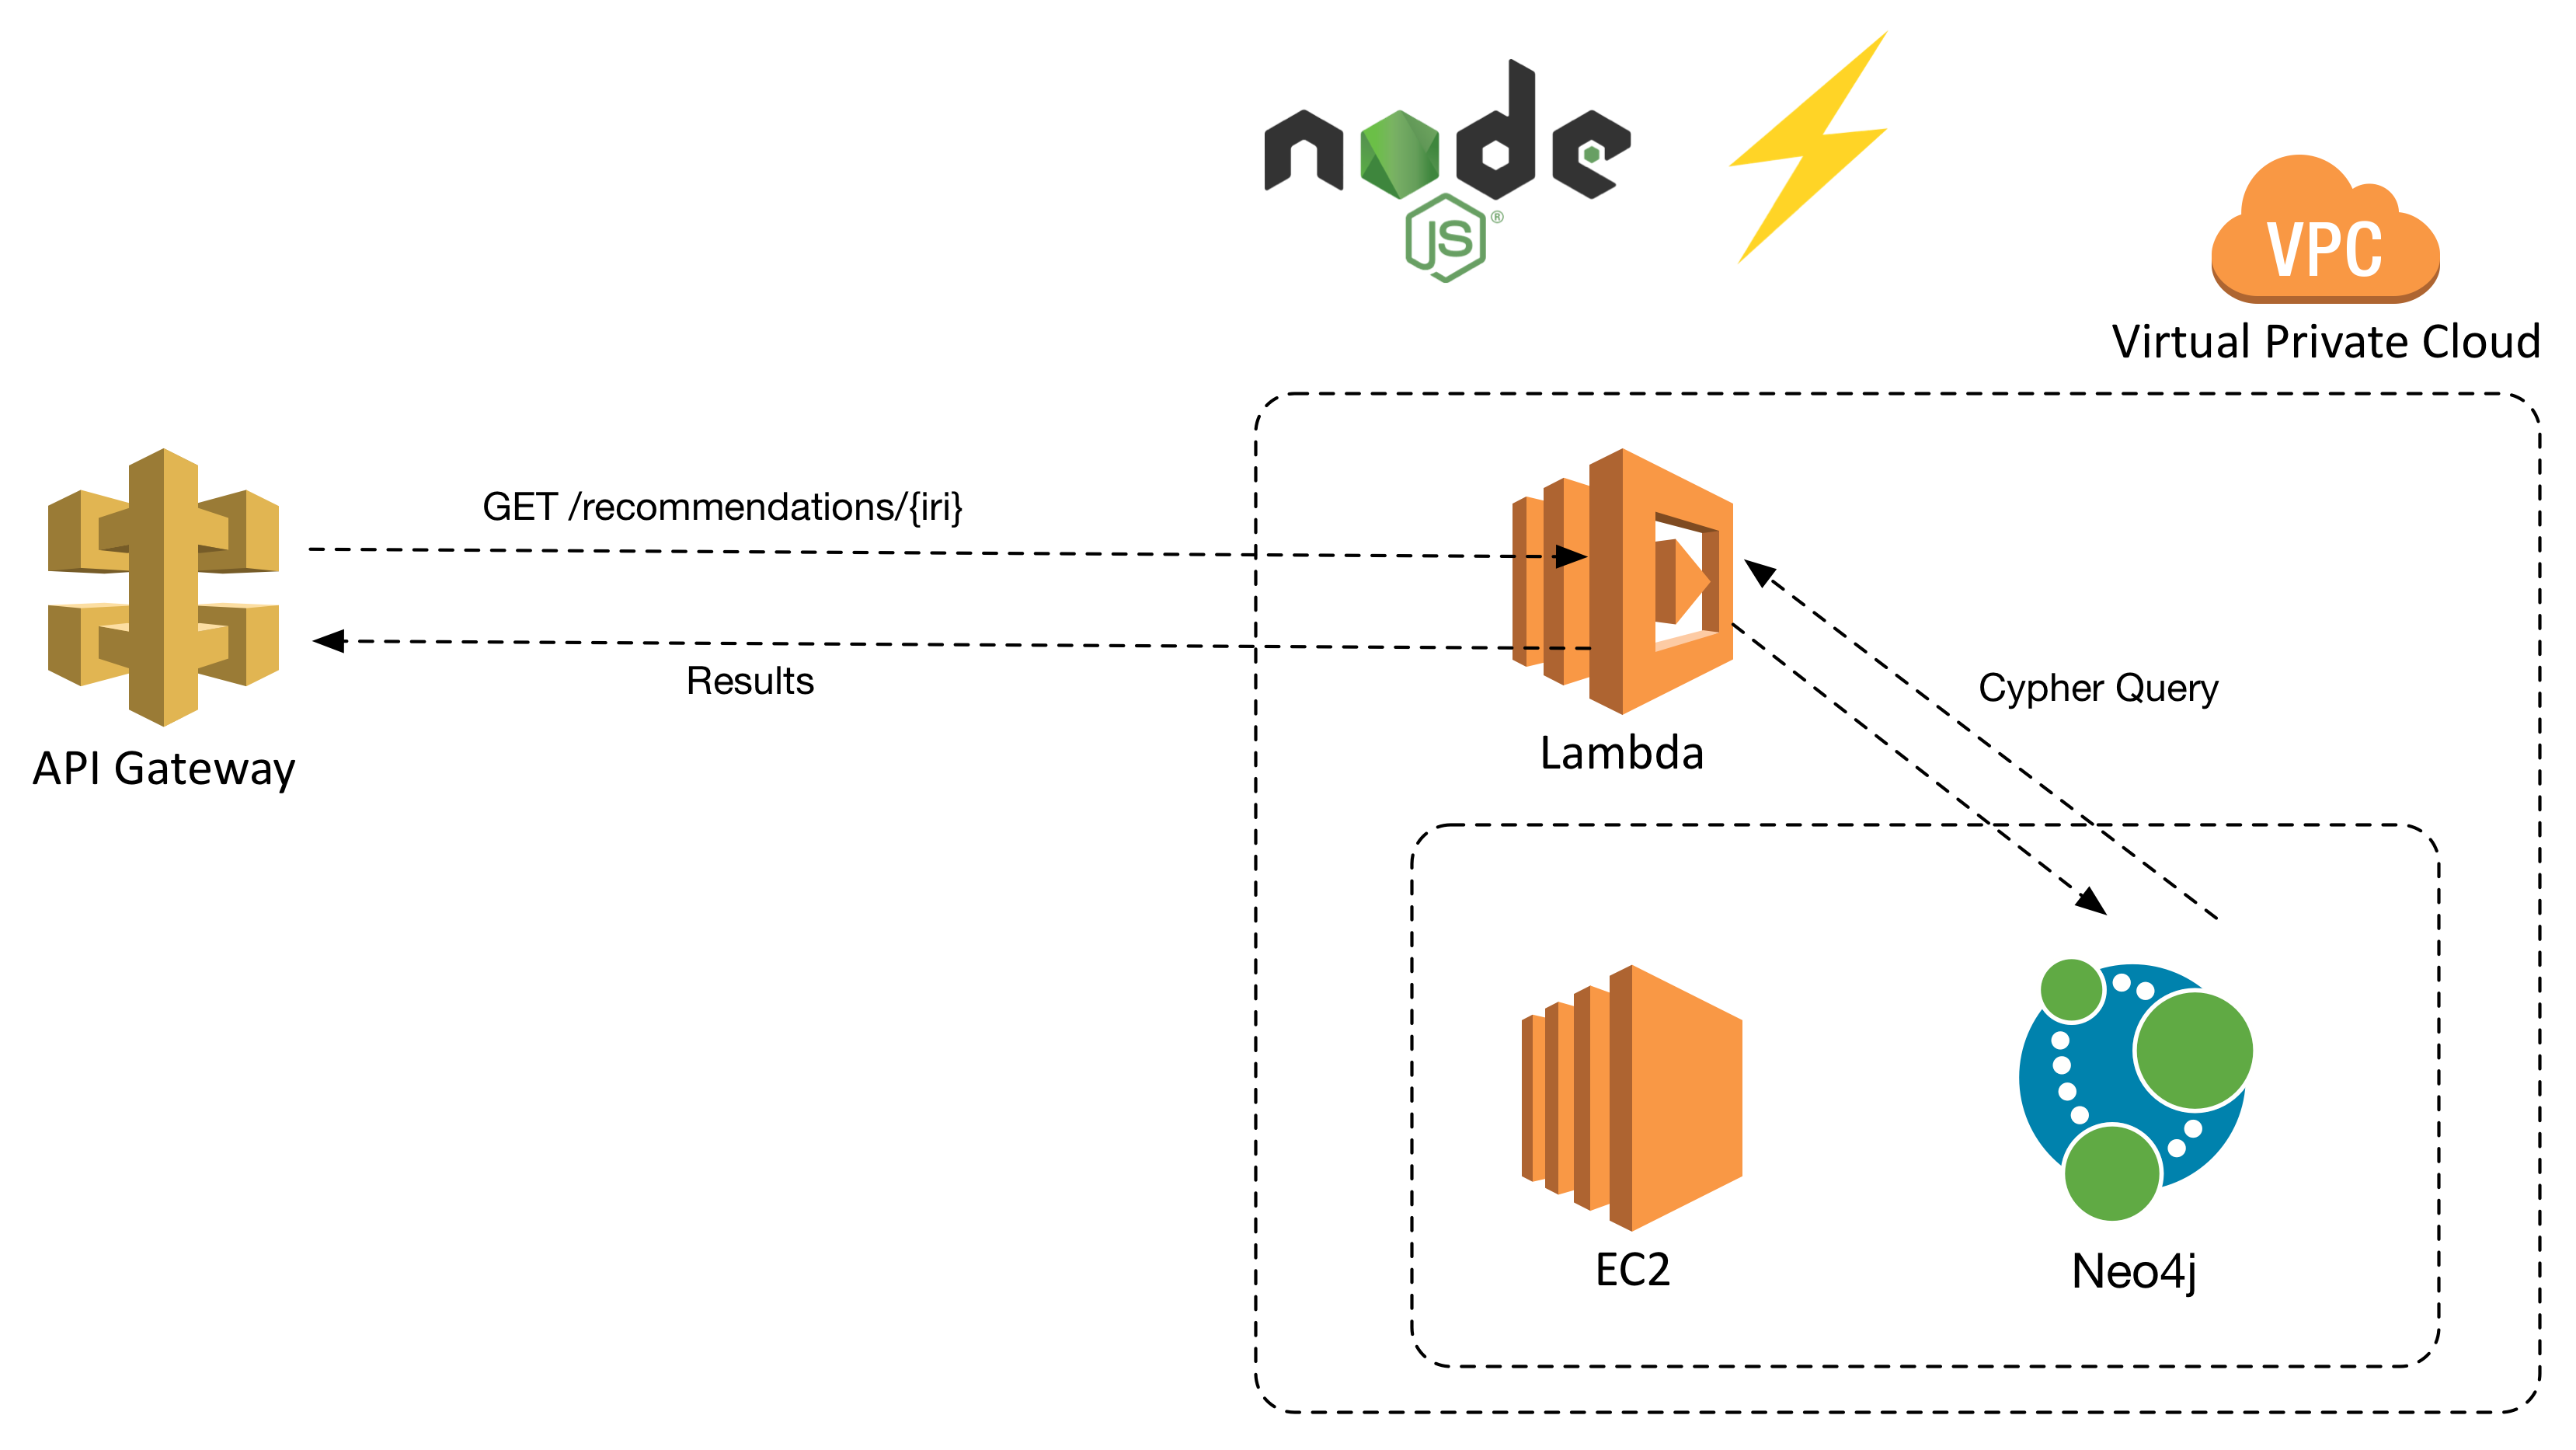
\includegraphics[width=0.7\textwidth,angle=0]{abb/Architecture}
 \caption[Beschreibung]{Architektur}
\label{fig:Architektur}
\end{figure}

Nachdem nun alle Komponenten eingerichtet sind erfolgt das Implementieren der Algorithmen und Datenbankabfragen. Als Laufzeitumgebung für die Lambda Funktionen wird Node.js in der Version 6.10 gewählt. Für die Anbindung an die Neo4j wird die \textit{neo4j-driver} Bibliothek geladen. Damit lässt sich zunächst für den gesamten Scope der Lambda Funktion der Datenbanktreiber der \textit{neo4j} Klasse instanzieren. 
Wird nun beim ausführen des Codes durch Lambda die \textit{Handler} Funktion aufgerufen, kann für den jeweiligen Handler eine neue Session geöffnet werden und ein String für die Datenbankabfrage, inklusive Parameter geformt werden. Ist die Abfrage beendet wird die Callback Funktion aufgerufen und ein Response Objekt erstellt, welches das Ergebnis der Datenbankabfrage im JSON String Format enthält.

Die Im Entwurf beschriebene Kern Komponente für die Datenbankanbindung, die Ein- uns Ausgabe von Daten und die Implementierung von Algorithmen, soll nun Lambda Funktionen in einer Node.js Laufzeitumgebung implementiert werden. Als erstes wird eine Instanz des Datenbanktreibers erzeugt welche von mehreren Handlern benutzt werden kann. Für jede Anforderung der Engine, soll ein eigener Handler implementiert werde, der genau dann ausgeführt wird wenn ein HTTP Request auf dem zu dem Handler gehörenden Pfad aufgerufen wird. Parameter aus dem Query String, oder Daten die mittels POST übermittelt werden können aus dem \textit{event} Objekt gelesen werden. 
\newline

Innerhalb des Handlers wird ein \textit{session} Objekt erzeugt, welches die Verbindung zur Datenbank herstellt und über diese auch die Abfragen an die Datenbank erfolgen. Dazu wird die \textit{run} Methode auf dem Objekt aufgerufen und der Querystring und Queryparameter übergeben. Es wird ein Promises erzeugt, auf welchem eine Callbackfunktion aufgerufen wird sobald die Abfrage alle Ergebnisse geliefert hat. Aus dem Resultset kann ein Objekt erzeugt werden welches mit der \textit{callback} Funktion des Lambda Handlers an den Aufrufer, in diesem Fall die API zurück gegeben wird.

Mit dem folgenden Handler wird ein Node \textit{n} über ein eindeutiges Attribut wie einer Id oder eines IRI in der Datenbank abgefragt und an die API zurückgeliefert.


\begin{lstlisting}[language=JavaScript, frame=htrbl, caption={Lambda Handler Funktion}, label={lst:lambda_handler}]
	'use strict';

var neo4j = require('neo4j-driver').v1;

var driver = neo4j.driver("bolt://"+process.env.NEO4J_URL, neo4j.auth.basic("user" ,"password"));
module.exports.getNode = function(event, context, callback) {
  var session = driver.session();
  session
  .run('MATCH (n:{queryParam}) return n;', {queryParam: event.queryStringParameters.label})
  .then(function (result) {
    result.records.forEach(function (record) {
      callback(null, {
        statusCode: 200,
        body: JSON.stringify({
          message: record,
          input: event,
        }),
      });
    });
    session.close();
    driver.close();
  })
  .catch(function (error) {
    console.log(error);
  });
};


\end{lstlisting}


\subsection{Deployment mit dem Serverless Framework}

Beim Erzeugen eines neuen Projektes mit dem Serverless Framework, wird neben einem leeren Handler auch eine Konfigurationsdatei mit dem Namen \textit{serverless.yaml} erzeugt. In dieser werden neben der Route die die Funktion auslöst auch die Art der HTTP Methoden eingetragen.

\begin{lstlisting}[language=Python, frame=htrbl, caption={Serverless Konfiguration}, label={lst:serverless_yaml}]

  functions:
  	getNode:
    	handler: handler.getNode
    	events: 
          - http: 
            	path: node 
         		method: get 
         		
\end{lstlisting}

Die notwendigen Paketabhängikeiten für die Datenbankanbindung an Neo4j werden mit \textit{npm install} in den node modules Ordner geladen. Über das Serverless Kommandozeilen Programm, wird mit dem \textit{deploy} Aufruf der gesamte Inhalt des Projektes, inklusive Abhängigkeiten gepackt, Cloudformation Templates erstellt und dann auf ein S3 Bucket in der AWS Cloud geladen. 

\subsection{Algorithmen und Metriken}

Das technische Gerüst ist nun komplett. Kompetenzen können per GET Request an die API, und unter Angabe ihrer IRIs abgefragt werden. Jedoch sind die Anforderungen an das Empfehlungssystem mittels Metriken und Algorithmen Ähnlichkeiten zu bestimmen. 

\subsubsection{Shortest Path}

Neo4j bringt eine Implementierung von kürzesten Pfaden direkt von Haus aus mit. Dafür müssen in der \textit{MATCH} Klausel nur ein spezifischer Anfangsknoten \textit{s} und ein Endknoten \textit{t} abgefragt werden und diese beiden in der \textit{shortestPath} Funktion als Parameter übergeben. Wahlweise kann der Pfad, oder die Länge des Pfades zurückgegeben werden.
\newline

Als grobe Metrik kann die shortestPath Funktion dazu verwendet werden um heraus zu finden wie weit eine Kompetenz von einer anderen entfernt ist. Je näher, desto ähnlicher. 

\subsubsection{Jaccard Index}

Zunächst soll geprüft werden, ob es Knoten Typen und Beziehungen im Graphen gibt mit denen sich eine Schnittmenge für zwei Kompetenzen berechnen lässt. Dabei soll eine Kompetenz von außen über die API als Eingabe erfolgen und solche Kompetenzen die eine Schnittmenge mit der gegebenen haben in geordneter Reihenfolge zurückgegeben werden. Diese Metrik lässt sich mit einer Cypher Abfrage direkt implementieren ohne weiteren Code ausführen zu müssen. Dazu wird zunächst die Abfrage formuliert. 

\textit{Welche Kompetenzen haben wieviele gemeinsame Beziehungen vom selben Typ zur gegebenen Kompetenz}
\newline

Als erstes werden mit einer \textbf{MATCH} Klausel alle Knoten $c_{gesucht}$ gesucht, die neben dem gegebenen Knoten $c_{input}$ eine eingehende Beziehung zu einem Knoten $o$ vom Typ \texttt{ns4\_Occupation} haben und die Schnittmenge bilden. 
\newline

\begin{lstlisting}
MATCH (c:ns4_Skill {ns5_prefLabel:{queryParam})-[:ns5_related]->(o:ns4_Occupation)<-[:ns5_related]-(other:ns4_Skill)
\end{lstlisting}



Die Kompetenz aus dem Input wird mittels Parameter der Query übergeben und das Resultat des Patterns in den Variablen $c$, $o$, $other$  mit der \textbf{WITH} Klausel in den nächsten Query Teil weiter gereicht. Mit der Aggregatsfunktion \textbf{COUNT} wird dann der Betrag der Schnittmenge von Knoten vom Typ \texttt{ns4\_Occupation}, die eine eingehende Beziehung vom Typ \texttt{ns5\_related} von Knoten $c_{input}$ und Knoten $c_{gesucht}$ vom Typ \texttt{ns4\_Skill} haben. 
\newline

\begin{lstlisting}
MATCH (c:ns4_Skill {ns5_prefLabel:{queryParam})-[:ns5_related]->(o:ns4_Occupation)<-[:ns5_related]-(other:ns4_Skill)

WITH c, other, COUNT(o) AS intersection, COLLECT(o.ns5_prefLabel) AS i

\end{lstlisting}

Als nächstes müssen die beiden Mengen in seperaten Variablen $s1_{A}$ und $s2_{B}$ gespeichert werden,

\begin{lstlisting}
MATCH (c:ns4_Skill {ns5_prefLabel:{queryParam})-[:ns5_related]->(o:ns4_Occupation)<-[:ns5_related]-(other:ns4_Skill)

WITH c, other, COUNT(o) AS intersection, COLLECT(o.ns5_prefLabel) AS i
MATCH (c)-[:ns5_related]->(c_other:ns4_Occupation)

WITH c,other,intersection, i ,COLLECT(c_other.ns5_prefLabel) AS s1
MATCH (other)-[:ns5_related]->(oc:ns4_Occupation)

WITH c,other,intersection,i, s1, COLLECT(oc.ns5_prefLabel) AS s2

\end{lstlisting}

um dann mittels Listenfunktion \textbf{FILTER} die Vereinigungsmenge zu berechnen.
\vspace{1em}

\begin{lstlisting}[language=SPARQL, morekeywords={MATCH, WITH, COLLECT}]
MATCH (c:ns4_Skill {ns5_prefLabel:{queryParam})-[:ns5_related]->(o:ns4_Occupation)<-[:ns5_related]-(other:ns4_Skill)
WITH c, other, COUNT(o) AS intersection, COLLECT(o.ns5_prefLabel) AS i

MATCH (c)-[:ns5_related]->(c_other:ns4_Occupation)
WITH c,other,intersection, i ,COLLECT(c_other.ns5_prefLabel) AS s1

MATCH (other)-[:ns5_related]->(oc:ns4_Occupation)
WITH c,other,intersection,i, s1, COLLECT(oc.ns5_prefLabel) AS s2

WITH c,other,intersection,s1+filter(x IN s2 WHERE NOT x IN s1) AS union, s1, s2

RETURN c.ns5_prefLabel, other.ns5_prefLabel, s1,s2,intersection,((1.0*intersection)/SIZE(union)) 

AS jaccard ORDER BY jaccard DESC LIMIT 10

\end{lstlisting}


Der Quotient aus dem Betrag der Schnittmenge, und dem Betrag der Vereinigungsmenge ergibt dann den Jaccard Index und wird gemeinsam mit den Namens Attributen für die die Kompetenzen $c_{input}$ und $c_{gesucht}$  in, in sortierter Reihenfolge in der \textbf{RETURN} Klausel in das Ergebnis geschrieben.

\subsubsection{Simrank}

In der Arbeit \textit{SimRank: A Measure of Structural-Context Similarity} wird gemäß dem Ansatz \textit{Zwei Objekte sind ähnlich, wenn sie mit ähnlichen Objekten verknüpft sind} ein Algorithmus vorgestellt, welche Die Ähnlichkeit von Objekten berechnet die in einem strukturellen Zusammenhang stehen. Für einen Knoten $v$ in eimem gerichteten Graphen mit $G = (V,E) $ wird eine Liste $I(v)$ mit Knoten die eine eingehende Beziehung haben, und eine Liste $O(v)$ mit ausgehenden Beziehungen erstellt. Ausgehend von der Annahme, dass ein Objekt eine maximale Ähnlichkeit von 1 zu sich selbst hat, soll nun die Ähnlichkeit von jedem Objekt über die Beziehungen zum nächsten propagiert werden, 	

\subsubsection{Levensthein oder Edit-Distanz}

Die Edit-Distanz oder auch 


